\setcounter{page}{1}
\section*{Zielsetzung}
In dem Versuch $V64$ wird mittels eines \emph{Sagnac Interferometer}
der Brechungsindex $n$ von Luft und einer Glasplatte bestimmt.
Hierbei bietet ein Sagnac Interferometer den Vorteil, dass sich
die beiden Strahlen des Interfeometer die selbe Strecke zurücklegen.
Hierdurch ist das Sagnac Interfeometer stabiler gegen externe Störung
als bspw. ein Michelson Interfeometer.

\section{Theorie}
Der Brechungsindex $n$ wird in mit einem Interferometer mit Hilfe von
Interferenzeffekten bestimmt. Interferent entstehen durch
eine Phasendifferenz $\Delta\phi$ zwischen zwei kohärenten Lichtstrahlen.
Eine solche Phasendifferenz wird in Gasen und Festkörpern unterschiedlich erzeugt.

%Brechungsindex von Gasen
%Brechungsindex von Festkörpern(Glasen)
%Polarisation
\subsection{Beschreibung von Licht}

Licht kann als Elektromagnetische Welle beschrieben werden.
Weil der elektrische und magnetische Teil miteinander gekopplet sind, reicht
es für eine vollständige Beschreibung aus nur den elektrischen Teil zu betrachten.
Für monochromatisches Licht kann das Elektrischefeld $\vec{E}$ mathematisch beschrieben
werden als
\begin{equation*}
  \vec{E} = \vec{E_0} \map{exp}\left(i (\omega t-\vec{k}\vec{r})\right),
\end{equation*}
hierbei repräsentiert $\vec{E_0}$ die Polarisation des Feldes.
Bei der Überlagerung von zwei Wellen kann es nun zu Interferenzeffekten kommen.
Hierbei gilt im allgemein für die Überlagerungsintensität
\begin{align}
  \label{eq:Interferenz_enstehung}
  \begin{aligned}
  \vec{E}_1&=\vec{E_{0,1}} \map{exp}\left(i (\omega t-\vec{k}\vec{r})\right) \qquad \vec{E}_2 =\vec{E_{0,2}} \map{exp}\left(i (\omega t-\vec{k}\vec{r}+\Delta\phi)\right) \\
  I &\propto \left<\be{E_1+E_2}^2\right> = E_{0,1}^2 + E_{0,2}^2 + 2E_{0,1}E_{0,1}\cos(\delta)\cos(\Delta\phi),
\end{aligned}
\end{align}
wobei $\Delta\phi$ die Phasendifferenz zwischen $\vec{E_1}$ und $\vec{E_2}$ darstellt und
$\delta$ der Polarisationswinkel der beiden Felder repräsentiert.
Die Art der Interfernz hängt somit von der Phasenverschiebung ab:
\begin{align}
  \Delta\phi &=0,2\pi,4\pi,\dots \qquad \text{Konstruktive Interfernz} \label{eq:Konstruktive}\\
  \Delta\phi &= \pi, 3\pi, 5\pi,\dots \qquad \text{Destruktive Interferenz}. \label{eq:Destruktive}
\end{align}
\subsection{Brechungsindex von Gasen}
Propagiert ein Lichtrahl von Medium $A$ durch eine Gasezelle der Länge $L$ mit Medium $B$,
so führt das zu einer Phasendifferenz $\Delta\phi$ relativ gesehen zu einem Lichtstrahl der sich
nur durch Medium $A$ bewegt. Erzeugt wird diese Phasendifferenz durch die Änderung der
Phasengeschwindigkeit im Medium $v\ua{ph}=\frac{\map{c}}{n_B}=\frac{\omega}{k}$, wobei $\map{c}$
die Vakuumlichtgeschwindigkeit repräsentiert. Eine Änderung der Phasengeschwindigkeit
verursacht eine Änderung der Wellenzahl $k$ und somit eine Phasenverschiebung
\begin{equation}
  \label{eq:phase_shit_gases}
\Delta\phi = kL = \frac{2\pi}{\lambda\ua{vac}}(n_B-n_A)L,
\end{equation}
mit der Vakuumwellenlänge $\lambda\ua{vac}$ und den Brechungsindizies der
Medien $A$ und $B$.
Zu beachten ist, dass der Brechungsindex eines Gases allgemein von dem Druck abhängt.
Die Abhängigkeit wird in einem Interferometer verwendet,um zwei kohärente Strahlen
interfiereren zu lassen.
Durch eine Beobachtung bzw. Zählung der Interferenzmaxima $M$ bei einer gegebenen Druckdifferenz
ist es möglich den Brechungsindex zu bestimmen.
\textbf{Lorentz-Lorenz Kurve}

\subsection{Brechungsindex von Festkörpern}
Im Gegensatz zu Gasen ist der Brechungsindex eines Festkörpers nicht Druckabhaängig.
Deshalb wird hier eine andere Bestimmungsmöglichkeit verwendet.
Propagiert ein Lichtstrahl, wie in Abbildung \ref{fig:slag} gezeigt durch einen Festkörper der Länge $T$,
so wird dieser nach dem Snelliussches Brechungsgesetz gebrochen.
\begin{figure}
\centering
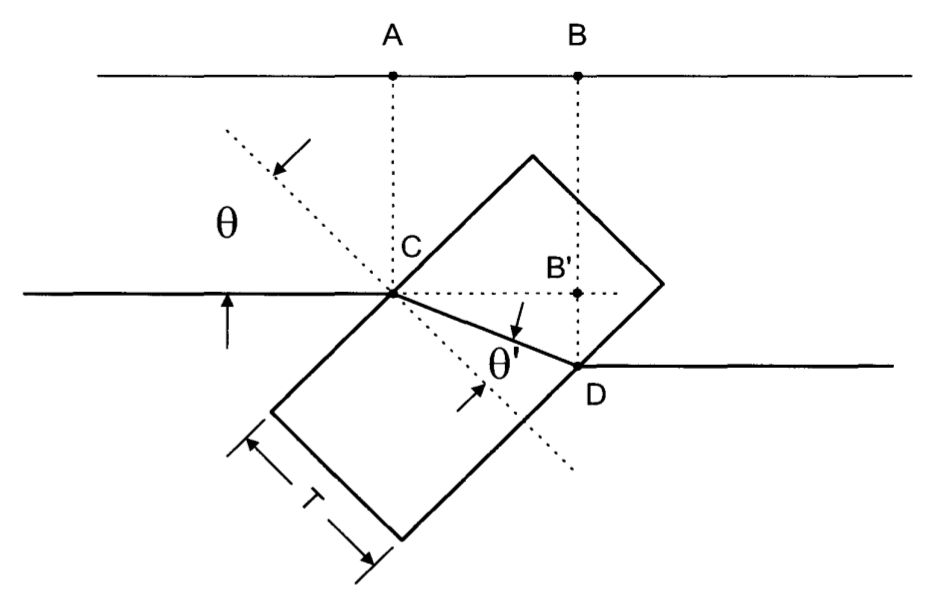
\includegraphics[width=0.7\linewidth]{./content/images/slab.png}
\caption{Ein Lichtstahl propagiert durch einen Festkörper z.\,B. Glas der Länge $T$ \cite{anleitung64}.}
\label{fig:slag}
\end{figure}
Hierdurch entsteht ein Gangunterschied der sich in eine Phasendifferenz übersetzt.
Mathematisch bestimmt werden kann die Phasendifferenz über den folgenden Zusammenhang
\begin{equation}
  \label{eq:Phasendifferenz_festkörper}
  \Delta\phi=\frac{ 2\pi T }{ \lambda\ua{vac} }\left( \frac{ n-\cos(\theta-\theta') }{ \cos(\theta') } - n+1\right),
\end{equation}
wobei $n$ der Brechungsindex des Festkörpers repräsentiert.
\textbf{TAylorentwicklung}
Mit der Phasendifferenz ist es nun möglich die Anzahl an Interfernzmaxima $M$ anzugeben, die bei einer Änderung
des Festkörpers um den Winkel $\theta$ entstehen. Zu beachten ist, dass der Laserstrahl zweimal den Festkörper
durchquert.
\begin{equation}
  \label{eq:Interferenzmaxima_solid_state}
  M=2\frac{\Delta\phi}{2\pi}=\textbf{HierNochTaylorentwicklungEinfügen}
\end{equation}
Wird die Gleichung \eqref{eq:Interferenzmaxima_solid_state} nach dem Brechungsindex $n$
umgestellt, ist es möglichen diesen aus $M$ zu bestimmen.
\begin{equation}
  \textbf{HiernochdieNeueFormeleinfügen}
\end{equation}

\subsection{Polarisation}
Bisher wurde nur der Wellencharakter von Licht betrachtet. Jedoch besitzt eine
Elektromagnetische Welle einen weiteren Freiheitsgrad, die Polarisation.
Die Polarisation gibt die Richtung des Elektrischenfeld Vektor an.
Eine Änderung der Polarisation kann mit Hilfe von Polarisationsfiltern bewirkt werden.
Der Filter absorbiert den Lichtanteil, welcher um $\frac{pi}{2}$ zum eingestellt Filterwinkel
gedreht ist. Somit wird das transmitierte Licht auf die Filterachse projiziert.

Zusätzlich werden in dem Versuch \emph{polarizing beam-splitter cubes} (PBSCs) verwendet.
Hergestellt wird ein solche Würfel, wenn zwei $45-45-\SI{90}{\degree}$ Prismen
an der Hypotenuse mit einander verklebt werden. Wichtig ist das auf dieser, vor dem verkleben,
eine dielekrische Schicht aufgebracht wird. Ein PBSC teilt den auftrefenden Strahl
in zwei Strahlen auf, die orthogonal in Ausbreitungsrichtung und Polarisation
sind (vgl. Abb. \ref{fig:pbsc}).
\begin{figure}
\centering
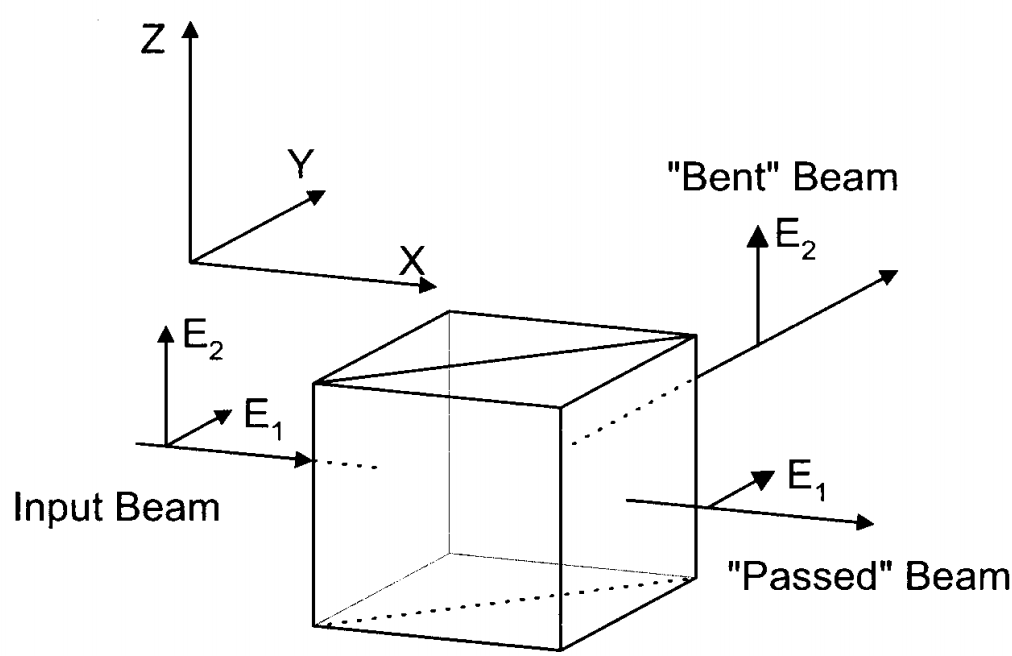
\includegraphics[width=0.7\linewidth]{./content/images/pbsc.png}
\caption{Schematische Darstellung eines PCBS \cite{anleitung64}.}
\label{fig:pbsc}
\end{figure}
